% Member 2 (Lucas) - Part 1 (c), (d), (e): distributions, maximum N, limit N ~ 10^23
% Figures: figures/omega_distributions.pdf, figures/probability_narrowing.pdf
\subsection{Distribution of Microstates}

The number of microstates with $k$ heads is the binomial coefficient:

\[
\Omega(N,k)=\binom{N}{k}=\frac{N!}{k!\,(N-k)!}
\]

To compute it, we cancelled the $(N-k)!$ and used the product
$\Omega(N,k)=\prod_{i=1}^{k}\frac{N+1-i}{i}$, which avoids calculating
very large factorials.
For large $N$ we used $\ln\Omega$, computed with the log-gamma function.

\begin{figure}[htbp]
  \centering
  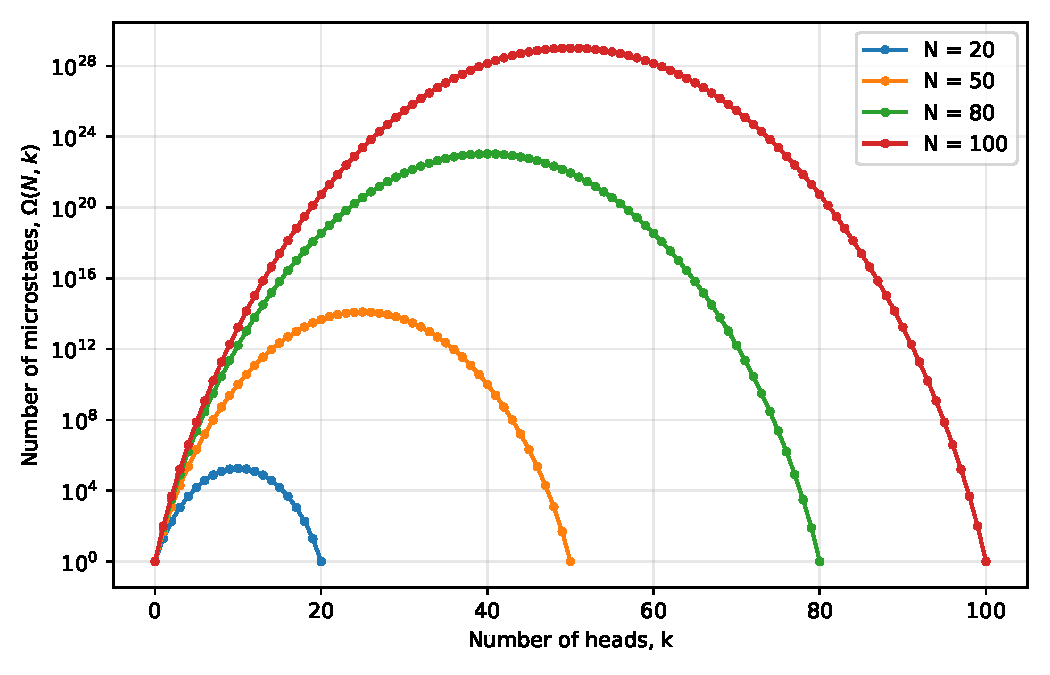
\includegraphics[width=0.7\linewidth]{figures/omega_distributions.pdf}
  \caption{$\Omega(N,k)$ for $N=20, 50, 80, 100$ (logarithmic scale).}
\end{figure}

All curves have their maximum at $k=N/2$ and are equal to 1 at $k=0$ and
$k=N$. The maximum grows very fast: about $10^5$ for $N=20$ and $10^{29}$ for
$N=100$.


\subsection{Maximum N}

\begin{itemize}
    \item Exact calculation: no limit, but it gets slower
    ($0.073 \pm 0.005$ s for $N=1000$, $3.24 \pm 0.04$ s for $N=4000$).

    \item Plotting: the largest number a computer float can store is about
    $1.8\times10^{308}$, so the maximum $N$ we can plot is $N=1029$.
\end{itemize}

Using $\ln\Omega$ instead removes this limit.


\subsection{Limit $N \sim 10^{23}$}

For large $N$ the distribution becomes a Gaussian with width
$\sigma=\sqrt{N}/2$, so the relative width is:

\[
\frac{\sigma}{N/2}=\frac{1}{\sqrt{N}}
\]

\begin{figure}[htbp]
  \centering
  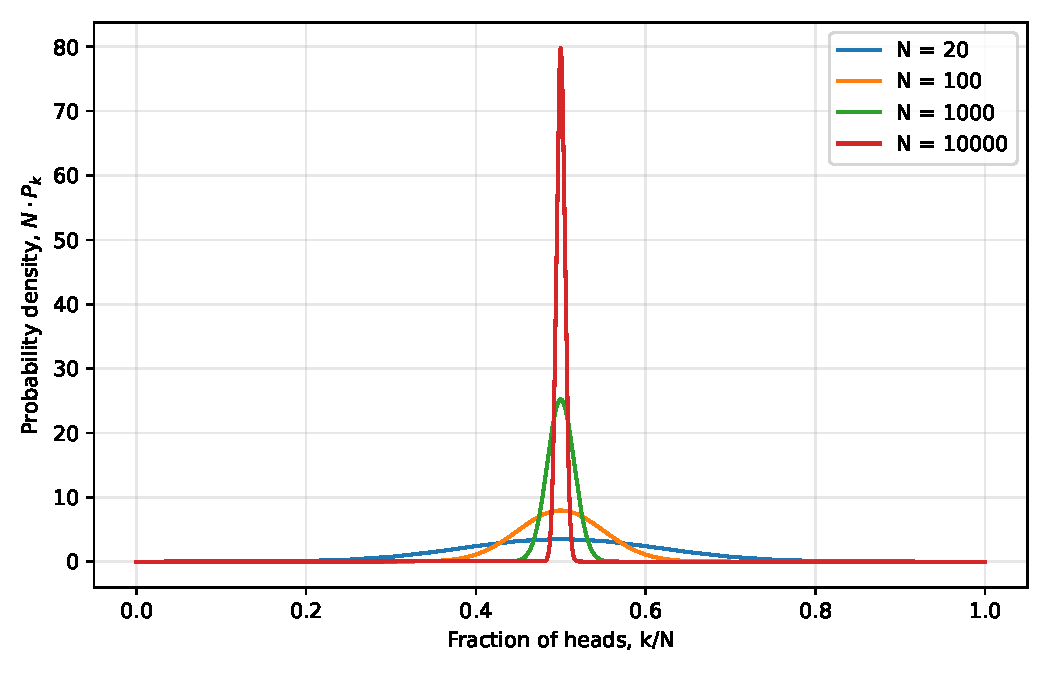
\includegraphics[width=0.7\linewidth]{figures/probability_narrowing.pdf}
  \caption{Probability versus fraction of heads $k/N$. The peak gets narrower
  as $N$ grows.}
\end{figure}

For $N=10^{23}$ the relative width is about $3\times10^{-12}$, so the
distribution is a very sharp peak at $k=N/2$. This means a macroscopic system
is practically always in the most disordered state.
\end{document}
 
